\documentclass[a4paper,doc,11pt]{article}
%----------------------------------------------------------------------------------------
%	Paquetes y configuraciones
%----------------------------------------------------------------------------------------
\usepackage[numbers]{natbib}
\bibliographystyle{apalike}

\usepackage{amsfonts}
\usepackage{amsmath}
\usepackage{amssymb,amsthm}
\usepackage{enumerate}
\usepackage{enumitem}
\usepackage[utf8]{inputenc}
\usepackage[T1]{fontenc}
\usepackage{geometry}
\usepackage{hyperref}
\geometry{left=2cm,right=2cm,top=2.5cm,bottom=2.5cm}



\usepackage{url}
\def\UrlBreaks{\do\/\do-}
\usepackage{multirow}
\usepackage{multicol}
\usepackage{enumitem}
\usepackage{nicefrac}
\usepackage{graphicx}
\usepackage{stmaryrd}
\usepackage{dsfont}
\usepackage{bropd}
\usepackage{easybmat}
\usepackage{setspace}
\usepackage{comment}
\usepackage{mathpazo}
\usepackage{array}
\usepackage{commath}

\usepackage{sectsty}
\sectionfont{\centering\fontsize{13}{15}\selectfont}
\subsectionfont{\centering\fontsize{10}{10}\selectfont\scshape}

\newtheorem{theorem}{Theorem}[section]
\newtheorem{corollary}{Corollary}[theorem]
\newtheorem{proposition}{Proposition}[theorem]
\newtheorem{lemma}[theorem]{Lemma}
\newtheorem{definition}[theorem]{Definition}
\newtheorem{remark}[theorem]{Remark}
\newtheorem{example}[theorem]{Example}
\newtheorem{claim}{Claim}[subsection]




\usepackage[font=small]{caption}
\usepackage[font=small]{subcaption}
\captionsetup{subrefformat=parens}
\usepackage{booktabs} % nice headers for tables

\newcommand{\R}{\mathbb{R}}
\newcommand{\Z}{\mathbb{Z}}
\newcommand{\N}{\mathbb{N}}
\newcommand{\CC}{\mathcal{C}}
\newcommand{\llb}{\llbracket}
\newcommand{\rrb}{\rrbracket}

\DeclareMathOperator{\dom}{dom}
\DeclareMathOperator{\dist}{dist}
\DeclareMathOperator{\supp}{supp}
\setcounter{MaxMatrixCols}{20}


\SetLabelAlign{parright}{\parbox[t]{\labelwidth}{\raggedright#1}}
\allowdisplaybreaks


\usepackage[symbol]{footmisc}

\renewcommand{\thefootnote}{\fnsymbol{footnote}}


\linespread{1.38}

%---------------------------------------- Autoría ---------------------------------------- %
\usepackage{titling}
\predate{}
\postdate{\vspace{-2\baselineskip}}



\title{\bf
    \Large
    SMSTC 2021 
    \\
    Variational Methods of PDEs
}
\author{}%Andrés Miniguano Trujillo}
\date{}


\begin{document}
%\pagenumbering{Roman} 
\maketitle




%\newpage
%\tableofcontents


%%%%%%%%%%%%%%%%%%%%%%%%%%%%%%%%%%%%%%%%%%%%%%%%%%%
%\newpage
\setcounter{section}{5}
\section{Young measures}
%\pagenumbering{arabic}

%%%%%%%%%%%%%%%%%

The first half of this course centred on the study of nonlinear functionals \(I(u)\) over a function space \(X\). For instance, in \(W^{1,p}(\Omega)\), we proved the existence of minimisers for \(I(u) = \int\limits_\Omega f(x,\nabla u)  \dif x\) whenever \(I\) is weak* lower-semicontinuous, and \(f\) is convex, which let us approach the problem of finding minimisers of \(I\) through the direct method of calculus of variations.

For instance, if we consider \( \Omega = (0,1)\), and the function \(f (\od{ }{x} u) = \big( (\od{ }{x} u)^2 -1 \big)^2\), then \(I(u) = \int\limits_\Omega f (\od{ }{x} u) \dif x\) attains a minimum over \(X = W^{1,4}_0(\Omega)\) and minimisers are functions such that \(\od{ }{x} u \in \{\pm 1\}\). It turns out that there are a infinite number of minimisers! To see this consider a sequence of saw-tooth functions as in Figure \ref{fig:6a}. There we can see that each function presents \(\od{ }{x} u \in \{\pm 1\}\) almost everywhere.

\begin{figure}
    \centering
    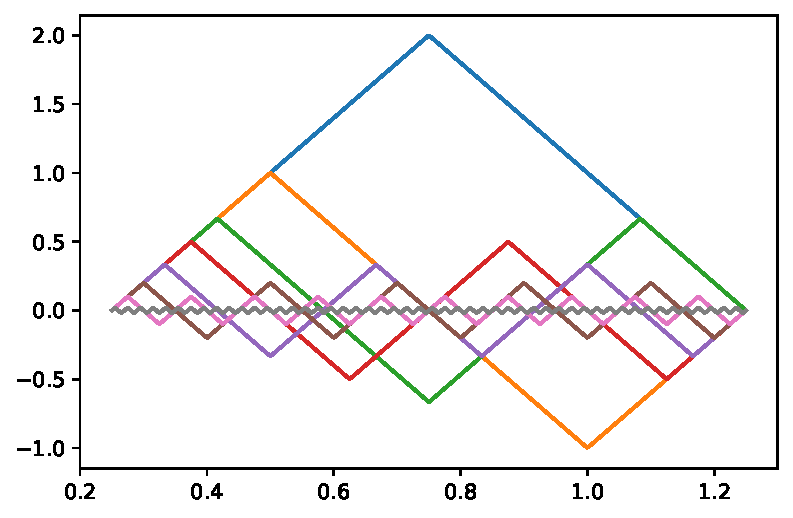
\includegraphics[scale=0.75]{Fig-6a.pdf}
    \caption{Saw-tooth functions}
    \label{fig:6a}
\end{figure}

Now consider the perturbed problem \( I(u) + \int\limits_\Omega |u|^2 \dif x \). We know that \( \inf I + \int |u|^2 = 0\); however, there does not exist minimisers for this function in the classical sense as a potential minimiser has to satisfy \(\od{ }{x} u \in \{\pm 1\}\) and \(u = 0\). In contrast, we can see that the saw-tooth sequence we used for \(I\) is minimising the perturbed problem, but its limit is not clear. In these lesson, we will focus on how to make sense of \emph{a function of slope \(\pm 1\) almost everywhere which is also \(0\) almost everywhere}. The answer is to use Young measures.

%Now we turn into giving sense to this behaviour among minimising sequences.

%%%%%%%%%%%%%%%%%
\subsection{Giving sense to minimising sequences}

Let us define \(C_0(\R^d)\) as the closure of continuous functions on \(\R^d\) with compact support. Its dual can be identified with the space of signed Radon measures with finite mass \(\mathcal{M}(\R^d)\) with the pairing
\[
    \langle \mu,f \rangle = \int_{\R^d} f \dif \mu.
\]
A map \(\mu : E \to \mathcal{M}(\R^d)\) is called weak* measurable if the functions \(x \mapsto \langle \mu(x), f\rangle\) are measurable for all \(f\in C_0 (\R^d)\). Here we will often write \(\mu_x\) instead of \(\mu(x)\).

\begin{theorem}[Fundamental theorem on Young measures]
    Let \(E \subset \R^d\) be a measurable set of finite measure, and let \(z_n : E \to \R^d\) be a sequence of measurable functions. Then there exists a subsequence \((z_{n_k})_{n_k \in \N}\) and a weak* measurable map \(\nu: E \to \mathcal{M}(\R^d)\) such that the following holds:
    
    \begin{enumerate}
        \item \(\nu_x\geq 0\) and \( \|\nu_x\|_{\mathcal{M}(\R^d)} = \int_{\R^d} \dif \nu_x \leq 1 \) for almost everywhere \(x\in E\).
        
        \item For all \(f \in C_0(\R^d)\)
        \[
            f(z_{n_k}) \overset{*}{\rightharpoonup} \overline{f}    \qquad \text{in } L^\infty (E)
        \]
        where
        \[
            \overline{f}(x) = \langle \nu_x,f \rangle.
        \]
        
        \item Let \(K \subset \R^d\) be compact, then 
        \[
            \supp(\nu_x) \subset K
            \qquad\text{if}
            \quad
            \dist(z_{n_k}, K) \to 0
            \quad
            \text{in measure}.
        \]
        
        \item Furthermore, one has that 
        \begin{equation}
        \label{measure:cond}
            \|\nu_x\|_{\mathcal{M}} = 1 \qquad \text{for almost everywhere } x\in E
            \tag{$i'$}
        \end{equation}
            if and only if the sequence does not escape to infinity; i.e., if
            \[
                \lim_{M\to \infty} \sup_k \big| \big\{ |z_{n_k}| \geq M \big\} \big| = 0.
            \]
        
        \item If \eqref{measure:cond} holds, and if \(A \subset E\) is measurable, \(f \in C(\R^d)\), and 
        \[
            f(z_{n_k}) \text{ is relatively compact in } L^1(A),
        \]
        then
        \[
            f(z_{n_k}) \rightharpoonup \overline{f} \quad \text{in } L^1(A).
        \]
        
        \item If \eqref{measure:cond} holds, then point (3) is also sufficient.
    \end{enumerate}
    
    The map \(\nu: E \to \mathcal{M}(\R^d)\) is called the \emph{Young measure} generated by (or associated to) \((z_{n_k})_{n_k \in \N}\).
\end{theorem}
\begin{comment}
Let us consider the following application of the last property:

\begin{example}
    Let \( (z_n)_{n\in \N}\) be bounded in \(L^p\) and \(\big|f(s)\big|\leq C(1 + |s|^q)\) for \( q < p\), then \(f(z_{n_k}) \rightharpoonup \overline{f}\) in \(L^{\nicefrac p q}\). In particular, if \(p>1\), the choice \( f = \mathrm{id}\) yields
    \[
        z_{n_k} \rightharpoonup z,
        \qquad
        z(x) = \langle \nu_x , \mathrm{id} \rangle.
    \]
\end{example}
\end{comment}
\begin{proof}
    The basic idea is to pass from functions in \(\R^d\) to maps in \(\mathcal{M}(\R^d)\). Thus we will use limiting objects which do not take a precise function value at every point but a probability distribution of values.
    
    Define \(Z_{n}(x) := \delta_{z_n} (x)\). Then by definition \( \|Z_n(x)\|_{\mathcal{M}} = 1 \) and \(\langle Z_n(x), f\rangle = f\big(z_n(x)\big)\). Thus \( (Z_n)_{n\in\N}\) belongs to the space \(L^\infty_w\big( E; \mathcal{M}(\R^d) \big)\): the space of weak* measurable maps from \(E\) to \(\mathcal{M}(\R^d)\) that are essentially bounded. From functional analysis in \(L^p\) spaces, it turns out that this is the dual of \(L^1 \big( E; C(\R^d) \big)\), which is separable. The natural duality pairing between the two is given by
    \[
        \langle \mu, g \rangle = \int\limits_E \big\langle \mu(x), g(x) \big\rangle \dif x
    \]
    Hence, the Banach-Alaoglu theorem\footnote{\emph{The closed unit ball of the dual space of a normed vector space is compact in the weak* topology.}} yields a subsequence such that
    \[
        Z_{n_k} = \delta_{n_k} \overset{*}\rightharpoonup \nu 
        \qquad\text{in } L^\infty_w\big( E; \mathcal{M}(\R^d) \big).
    \]
    Moreover, as the norm is lower-semicontinous, we have that \(\|\nu_x\|_\mathcal{M} \leq 1\) for almost everywhere \(x\). 
    
    For \(\varphi \in L^1(E)\) and \(f\in C_0(\R^d)\), let us denote \( \varphi \otimes f \) as an element of \(L^1 \big( E; C(\R^d) \big)\) such that \( x \mapsto \varphi(x) f\). By definition of \((Z_n)_{n\in \N}\) and the previous convergence result, we get
    \[
        \int\limits_E \varphi(x) f\big( z_{n_k}(x) \big) \dif x
        = \big\langle Z_{n_k}, \varphi \otimes f \big\rangle
        \to
        \int\limits_E \varphi(x) \langle \nu_x, f\rangle \dif x.
    \]
    This implies (2), and if we consider functions \( f\geq 0\) and \(\varphi \geq 0\), then \( \nu_x\geq 0\) follows as well, so we have (1) too.
    
    To proof (3), consider \(K\subset \R^d\) compact with \(\dist(z_{n_k}, K) \to 0\) in measure. Here it suffices to show that
    \begin{equation}
    \label{to-prove}
        \langle \nu_x , f\rangle = 0    \qquad \forall f \in C_0(\R^d \setminus K).
    \end{equation}
    Let \(f \in C_0(\R^d \setminus K)\), then for every \( \varepsilon >0\) there is \( c_\varepsilon\) such that \( \big| f(y) \big| \leq \varepsilon + c_\varepsilon \dist(y,K) \). Hence, by hypothesis \(\dist(z_{n_k}, K) \to 0\) implies that \( \big( |f| - \varepsilon \big)^+ (z_{n_k}) \to 0 \) in measure, but property (2) yields that
    \[
        \big\langle \nu_x ,  \big( |f| - \varepsilon \big)^+ \big\rangle = 0
    \]
    for almost everywhere \(x\), and as \(\varepsilon\) is arbitrary, we have that \eqref{to-prove} follows.
    
    To prove (4), let us start assuming that
    \[
        \|\nu_x\|_{\mathcal{M}} = 1 \qquad \text{for almost everywhere } x\in E.
    \]
    Let us argue by contradiction and suppose that there exists \( R>0\) and \(\varepsilon >0 \) such that there exists a sequence \(L_k\to \infty\) and integers \(n_k\) such that
    \[
        \big| \big\{x\in E \cap B_R:  |z_{n_k}|(x) \geq L_k \big\} \big| > \varepsilon.
    \]
    for all \(k \in \N\). For \(\rho>0\), consider the function
    \[
        \alpha_\rho (t) :=
        \begin{cases}
            1   &   \text{if } t \leq \rho,
            \\
            0   &   \text{if } t \geq \rho + 1,
            \\
            \rho + 1 -t & \text{if } t \in (\rho,\rho+1).
        \end{cases}
    \]
    Then the function \(\varphi_\rho:\R^d \to\R\) such that \( \varphi_\rho(x) = \alpha_\rho(|x|)\) is in \(C_0 (\R^d)\). By the second part of the theorem, we have that
    \[
        \int\limits_E \varphi_\rho (z_{n_k}) \chi_{B_R} \dif x
        \to
        \int\limits_E \langle \nu_x, \varphi_\rho \chi_{B_R}\rangle \dif x.
    \]
    Now, we find that for \(k\) large enough
    \[
        |E\cap B_R| - \varepsilon \geq \int\limits_E \varphi_\rho (z_{n_k}) \chi_{B_R} \dif x;
    \]
    and this implies
    \[
        |E\cap B_R| - \varepsilon \geq \int\limits_E \langle \nu_x, \varphi_\rho \chi_{B_R}\rangle \dif x.
    \]
    On the other hand, by the monotone convergence theorem, we conclude that the right-hand side of the latter expression converges as \(\rho\to \infty\) to 
    \[
        \int\limits_E \langle \nu_x, \chi_{B_R}\rangle \dif x
        =
        \int\limits_E \|\nu_x\|_{\mathcal{M}} \chi_{B_R} \dif x = |E \cap B_R|,
    \]
    which is a contradiction with the previous inequality.
    
    The converse is as follows: Let \(R>0\) be fixed and let \(f\equiv 1\) be a constant function in \(\R^d\). Then \(f(z_{n})\) is sequentially weakly relative compact in \(E \cap B_R\) and as the sequence \((z_{n_k})_{n_k\in \N}\) does not escape to infinity we get
    \[
        |E\cap B_R| = \int\limits_E f(z_{n_k}) \chi_{B_R} \dif x
        \to
        \int\limits_E \langle \nu_x, \chi_{B_R}\rangle \dif x
        =
        \int\limits_{E\cap B_R} \|\nu_x\|_{\mathcal{M}}  \dif x.
    \]
    Since \(\|\nu_x\|_{\mathcal{M}} \leq 1\), we conclude \( \|\nu_x\|_{\mathcal{M}} = 1\) a.e. \(x \in E\cap B_R\), and as \(R\) was arbitrary, the property follows.
            
    
    Now suppose that \eqref{measure:cond} holds, \(f \in C(\R^d)\), and that
    \(
        f(z_{n_k}) 
    \)
     is relatively compact in  \(L^1(E)\). Let \( f^+ = \max\{f,0\}\) and \( f^- = \max\{-f,0\}\). By Dunford-Pettis theorem\footnote{Suppose that \((X,\Sigma,\mu)\) is a probability space and that \(\mathcal{F}\) is a bounded subset of \(L^1(\mu)\). \(\mathcal{F}\) is equi-integrable if and only if \(\mathcal{F}\) is a relatively compact subset of \(L^1(\mu)\) with the weak topology.}, we get that \(f^+(z_{n_k})\) and \(f^-(z_{n_k})\) are both sequentially weakly relatively compact in \(L^1(E)\). Now, to prove (5) we will suppose that \(f\geq 0\), and that \(A\) is bounded with \( f(z_{n_k}) \rightharpoonup \mu\), in \(L^1(A)\). 
     
     Define \(f_\rho = \varphi_\rho f\) with \(\varphi_\rho\) the same function we defined above, and let \(\psi \in L^\infty (A)\). We claim that 
     \[
        \int\limits_A \psi f_\rho (z_{n_k}) \dif x
        \to
        \int\limits_A \psi f (z_{n_k}) \dif x
     \]
     as \(\rho \to \infty\), uniformly in \(n_k\). In fact
     \[
        \bigg|
        \int\limits_A \psi ( f_\rho - f) (z_{n_k}) \dif x
        \bigg|
        \leq c 
        \int\limits_{ \{x\in A: \, |z_{n_k}|(x) \geq \rho \} }  f (z_{n_k}) \dif x,
     \]
     and, given \(\varepsilon>0\), by the Dunford-Pettis theorem there exists an \(M>0\) such that
     \[
        \sup_{n_k} \int\limits_{ \{x\in A: \, |z_{n_k}|(x) \geq M \} }  f (z_{n_k}) \dif x \leq \varepsilon.
     \]
     This alongside the boundness condition in (4) yields the claim. Now, we also have
     \[
        \lim_{n_k \to \infty} \int\limits_A \psi f_\rho(z_{n_k}) \dif x
        = \int\limits_A \psi \langle \nu_x, f_\rho \rangle \dif x.
     \]
     Here it follows that
     \[
        \lim_{\rho \to \infty} \int\limits_A \psi \langle \nu_x, f_\rho \rangle \dif x
        = \int\limits_A \psi \mu \dif x.
     \]
     Choosing \(\psi \geq 0\) and noting that \( f_\rho\) is increasing,  we deduce from the monotone convergence theorem that \( \mu = \langle \nu_x, f\rangle\) as needed.
    
    Finally, the proof of (6) follows by applying (5) with the bounded function \(f = \max\{\dist(\cdot, K),1\}\).
\end{proof}

\begin{example}
    In the limiting case of Figure \ref{fig:6a}, \(\od{ }{x} u\) is the measure \( \nu_x = \frac 1 2 \delta_{-1} + \frac 1 2 \delta_{+1}\); moreover,  \(\supp(\nu_x) = \{\pm 1\}\). 
    
    Here we have that if \( f(z) = z\), then
    \[
        \langle \nu_x,f \rangle = \frac{1}{2} 1 + \frac{1}{2} (-1) = 0.
    \]
    Likewise, if \( f(z) = z^2\), then
    \[
        \langle \nu_x,f \rangle = \frac{1}{2} (1)^2 + \frac{1}{2} (-1)^2 = 1.
    \]
\end{example}

\begin{corollary}
    Suppose that a sequence \((z_n)_{n\in \N}\) of measurable functions from \(E\) to \(\R^d\) generates the Young measure \( \nu: E \to \mathcal{M}(\R^d)\). Then 
    \[
        z_n \to z \text{ in measure if and only if } \nu_x = \delta_{z(x)} \text{ a.e.}
    \]
\end{corollary}
\begin{proof}
    If \(z_n \to z\) in measure, then \( f(z_n) \to f(z)\) in measure as well for all \( f \in C_0(\R^d)\). Hence by (2) in the fundamental theorem one has that
    \[
        \langle \nu_x, f\rangle = f\big( z(x) \big)
    \]
    for all \( f \in C_0(\R^d)\) and thus \(\nu_x = \delta_{z(x)}\).
    
    Conversely, if we have that \(\nu_x = \delta_{z(x)}\) almost everywhere, we claim that
    \[
        \limsup_{n\to \infty} \big| \{|z_n -w | >\varepsilon\} \big|
        \leq 
        \big| \{|z_n -w | > \nicefrac{\varepsilon}{2}\} \big|
    \]
    for all piecewise constant measurable functions \(w:E\to \R^d\). To see this it suffices to consider constant functions \(w\equiv a\) and apply (5) from the fundamental theorem with \(f(y) = \varphi(|y-a|)\), with \(\varphi\) continuous \(0\leq \varphi \leq 1\), \(\varphi = 1\) on \([\varepsilon,\infty)\), and \(\varphi = 0\) on \([0,\nicefrac{\varepsilon}{2}]\). Thus
    \begin{align*}
        \limsup_{n\to \infty} \big| \{|z_n -z | >\varepsilon\} \big|
        &\leq
        \limsup_{n\to \infty} \big| \{|z_n -w | >\nicefrac{\varepsilon}{2}\} \big|
        + \big| \{|z -w | > \nicefrac{\varepsilon}{2}\} \big|
        \\
        &\leq 
        \big| \{|z -w | > \nicefrac{\varepsilon}{4}\} \big|.
    \end{align*}
    The last term can be made arbitrarily small since measurable functions can be approximated by piecewise constant functions, and the assertion follows.
\end{proof}

A key example for Young measures is the following, generalising \(\nu_x = \frac{1}{2} \delta_{-1} + \frac{1}{2} \delta_{+1}\) from our motivating problem.


\begin{example}
    Let \(h : \R \to \R\) be the periodic extension of the function given by
    \[
        h(x) = 
        \begin{cases}
            a & \text{if }x \in [0,\lambda),
            \\
            b & \text{if }x \in [\lambda,1),
        \end{cases}
    \]
    and define \(z_n : [0,1] \to \R\) by \( z_j(x) = h(jx)\). 
    
    Using the periodicity of \(h\), one arrives at
    \[
        z_n \overset{*}{\rightharpoonup} \int\limits_0^1 h(y) \dif y = \lambda a + (1-\lambda) b 
    \]
    or more generally 
    \[
        f(z_n) \overset{*}{\rightharpoonup} \lambda f(a) + (1-\lambda) f(b).
    \]
    As a result, \((z_n)_{n\in\N}\) generates the following Young measure:
    \[
        \nu_x = \lambda \delta_a + (1-\lambda) \delta_b,
    \]
    which is independent of \(x\). Such measures are called \emph{homogeneous Younge measures}.
\end{example}


%%%%%%%%%%%%%%%%%

A fundamental question for applications is now: Which \(\nu \in L^\infty_w (\Omega, \mathcal{M}(\R^d))\) are Young measures of \emph{gradients}?

\begin{definition}
    Let \(\Omega \subset \R^d\) denote a bounded domain with Lipschitz boundary.
    
    We say that a weakly* measurable map \(\nu: \Omega \to \mathcal{M}(M^{m\times d}) \) is a \(W^{1,p} \) gradient Young measure if there exists a sequence of maps \(u_n : \Omega \to \R^d\) such that
    \begin{align*}
        u_n &\rightharpoonup u
        \quad \text{in } W^{1,p} (\Omega, \R^m) \qquad (\overset{*}{\rightharpoonup}) \text{if } p = \infty),
        \\
        \delta_{Du(\cdot)} &\overset{*}{\rightharpoonup} \nu 
        \quad \text{in } L^\infty_w \big(\Omega, \mathcal{M}(M^{m\times d})\big).
    \end{align*}
\end{definition}

Now in turn we may consider the following problem:

\begin{quote}
    Given a set \(K \subset M^{m\times d}\), characterise all \(W^{1,\infty}\)-gradient Young measures \(\nu\) such that
    \[
        \supp(\nu_x) \subseteq K
        \qquad \text{for a.e. } x.
    \]
\end{quote}

This has implications for what kind of macroscopic properties a physical system can have. There is a classification due to \citet{Kinderlehrer1994}.



%%%%%%%%%%%%%%%%%%%%%%%%%%%%%%%%%%%%%%%%%
%%%%%%%%%%%%%%%%%%%%%%%%%%%%%%%%%%%%%%%%%
\section*{Further references}

Most of the notes here can be traced back to the book of \citet{Mueller-1999}. The proof of the fundamental theorem uses complementaty results from \citet{Hungerbhler2011} and \citet{Balla-1989}. A proof of Banach-Alaoglu theorem is also available at \citet{Brezis2010}.




%%%%%%%%%%%%%%%%%%%%%%%%%%%%%%%%%%%%%%%%%


\section*{Availability of data, material, and code}
{
%\small

All the files and this document are available as in the following repository:
\begin{quote}
    \noindent \href{https://github.com/andresrmt/Variational-Methods-for-PDEs}{\texttt{https://github.com/andresrmt/Variational-Methods-for-PDEs}}
\end{quote}



}

%%%%%%%%%%%%%%%%%%%%%%%%%%%%%%%%%%%%%%%%%
%%%%%%%%%%%%%%%%%%%%%%%%%%%%%%%%%%%%%%%%%
%\newpage


\bibliography{Cites}

\end{document}


Last week we saw that the functional 
\(
    I(u) = \int\limits_{[0,1]^2} u_x^2 + (u_y^2-1)^2 \dif x
\)
had zero as an infimum but could not attain a minimum. Namely, we built a sequence \((u_n)_{n\in \N}\) in \(H_0^1 (\Omega) \cap W_0^{1,4} (\Omega)\) such that \( J(u_n) \to 0\) and \(u_n \to 0\) in \(L^2(\Omega)\), but this resulted in a contradiction as \(J(0) = 1\). 
